\chapter{Dokumentation der Implementierung}
Im folgenden Kapitel wird eine detaillierte Beschreibung der wichtigen Funktionen geliefert. Zudem sind Code-Ausschnitte sowie Screenshots der einzelnen Funktionen zur besseren Verständlichkeit vorhanden. 

\section{Registrieren}
Das Fenster, um sich als Lieferant zu registrieren, kann über den Lieferanten-Login aufgerufen werden. Diese Funktion wird ausschließlich von Lieferanten in Anspruch genommen, die ihre zukünftigen Rechnungen auf die Plattform hochladen wollen. Beim Registrieren kann der Lieferant einen Benutzernamen, eine E-Mail-Adresse und ein Passwort, das den vorgeschriebenen Kriterien entspricht, eintragen. Zusätzlich muss er seine ELK Fertighaus GmbH interne Lieferantennummer angeben, um die Registrierung abschließen zu können. Diese Nummer kann er aus einer Liste auswählen, in der die Bezeichnung des Lieferanten zusätzlich zu der Lieferantennummer angegeben ist. Bei der Registrierung wird überprüft, ob die Form komplett ausgefüllt wurde, ob die beiden eingegebenen Passwörter übereinstimmen und infolgedessen, ob das Passwort den Passwortkriterien aus der Datenbank entspricht. Wenn ein Fehler bei der Registrierung auftritt, wird der Benutzer mit einer entsprechenden Fehlermeldung versorgt. Nach Abschluss der Registrierung erhält der Lieferant eine E-Mail, die bestätigt, dass er sich erfolgreich registriert hat. Weiters wird ein neuer Benutzer in der Datenbank angelegt und die Benutzer-ID dem zugehörigen Lieferanten zugewiesen. Das eingegebene Passwort wird mit einer Laravel internen Funktion\footnote{\url{https://laravel.com/docs/5.2/hashing}} verschlüsselt und so in die Datenbank geschrieben. Allerdings kann der Lieferant sich zu diesem Zeitpunkt noch nicht registrieren, da die Buchhaltung seinen Benutzer erst freischalten muss.
\newpage
Unten sehen Sie einen Ausschnitt aus der Registrier-Methode. Die Methode erstellt den Benutzer und prüft, ob die Lieferantennummer existiert. Wenn diese existiert, wird dem Lieferanten die zugehörige Benutzer-ID zugewiesen. Abschließend wird noch eine E-Mail an den Lieferanten versendet.

\lstset{language=PHP,caption={Registrier-Methode, für kompletten Ausschnitt siehe S. \pageref{regiscode}},label=registrieren}
\begin{lstlisting}
//Benutzer wird erstellt
$user = User::create(['username' => $username, 'password' => $password, 'changed_password_date' => Carbon::now(), 'has_changed' => '1', 'rights' => 'supplier', 'locked' => '1', 'email' => $email]);

//Prüfen, ob die eingegebene Firmennummer existiert
if (isset($company_id)) {
	//speichert die Benutzer-ID zum zugehörigen Lieferanten
	$supplier = Supplier::where('id', '=', $company_id)->first();
	$supplier->user_id = $user->id;
	$supplier->newregistered = 1;
	$supplier->save();
}

//E-Mail versenden
$this->sendMail($user, 'mail.registeredmail', 'Erfolgreich registriert:');
                
\end{lstlisting}

\newpage
In der Abbildung unten ist die Form für die Registrierung der Lieferanten zu sehen.
\begin{figure}[!h]
    \centering
    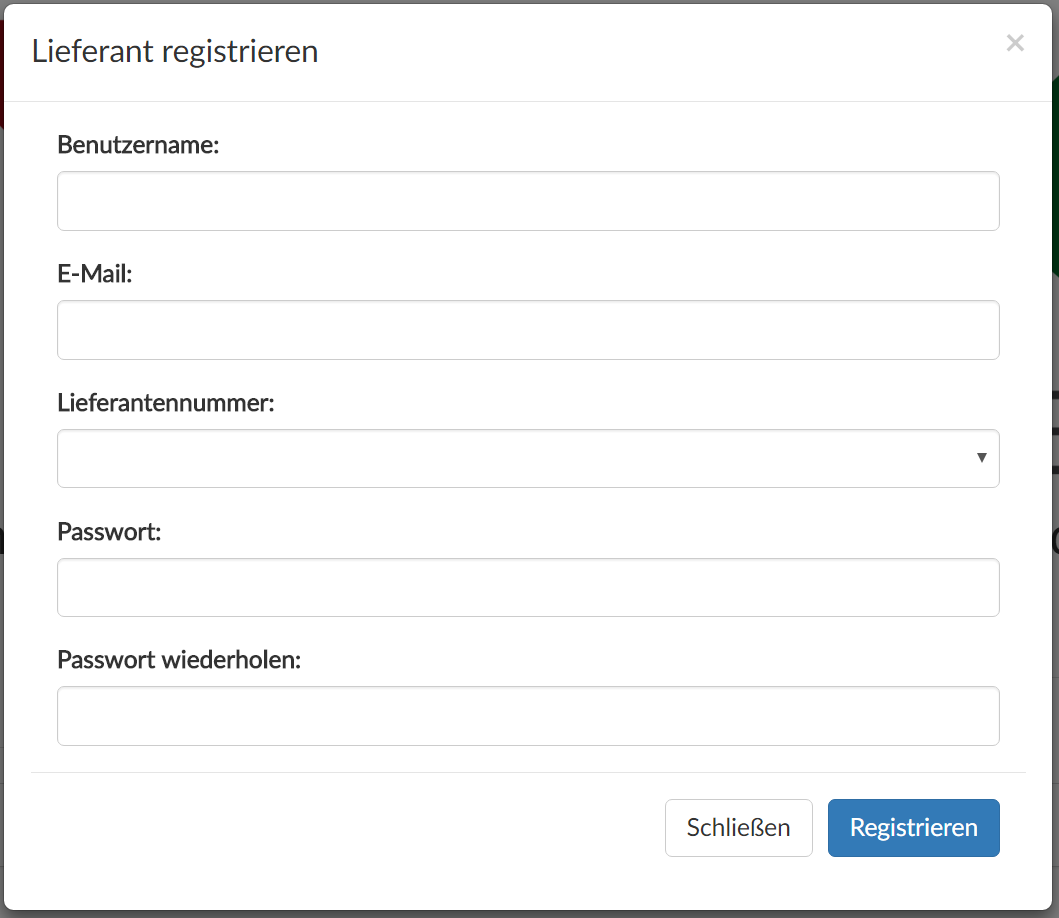
\includegraphics[width=17cm]{figures/registermock.png}
    \label{fig:takebill}
    \caption{Lieferant registrieren-Oberfläche}
\end{figure}

\newpage
In der unten stehenden Grafik ist das Ablaufdiagramm der Registrier-Funktion zu sehen.
\begin{figure}[!h]
    \centering
    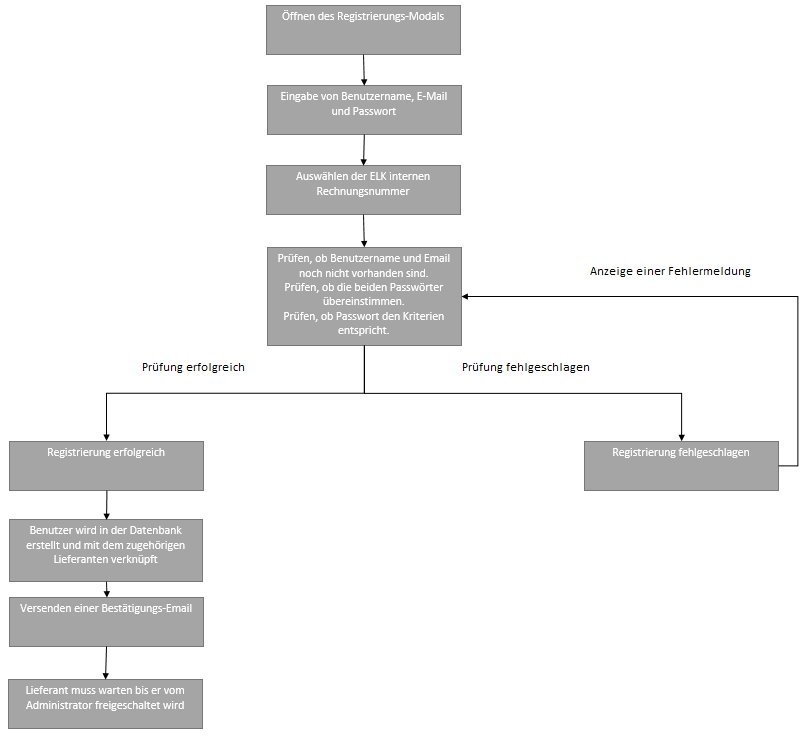
\includegraphics[width=17cm, height=18cm]{figures/register.png}
    \label{fig:register}
    \caption{Lieferant registrieren-Ablaufdiagramm}
\end{figure}
\newpage

\section{Login}
Die Plattform beinhaltet zwei unterschiedliche Login-Masken, wenn man die Startseite der elektronischen Rechnungsplattform betritt, zum einen den Lieferanten-Login und zum anderen den Buchhaltungs-/Administrator-Login. Wenn Benutzername und Passwort eingegeben wurden, wird auf deren Existenz und Gültigkeit mithilfe der Datenbank geprüft. Das Passwort wird zusätzlich verschlüsselt\footnote{\url{https://laravel.com/docs/5.2/hashing}} übertragen, um es mit dem aus der Datenbank vergleichen zu können. Danach wird untersucht, ob der Nutzer die jeweiligen Rechte für die Login-Maske besitzt, das bedeutet, dass der Lieferant den Lieferanten-Login benutzt. Beim Lieferant wird zusätzlich überprüft, ob seinem Benutzer ein Lieferant zugewiesen ist. Wenn eine der oben genannten Überprüfungen fehlschlägt, wird dem aktuellen Benutzer eine entsprechende Fehlermeldung angezeigt, die das aufgetretene Problem beschreibt. Falls der Login-Versuch erfolgreich durchgeführt wurde, wird eine Benutzer-Session erstellt und der Nutzer auf dessen jeweilige Seite weitergeleitet. (z.B.: Lieferant gelangt auf Lieferanten-Seite) Zudem wird überprüft, ob das Passwort des Benutzers geändert werden muss (z.B.: Passwortänderungsintervall wurde überschritten). Falls ja, wird der betreffende Nutzer direkt auf die Passwort ändern-Webseite weitergeleitet.

\newpage
Unten sehen Sie einen Ausschnitt aus der Login-Methode des Lieferanten. Es finden Überprüfungen statt, ob der Benutzer existiert, ob er gesperrt ist, ob er die Rechte eines Lieferanten besitzt. Dann wird das eingegebene Passwort verschlüsselt und mit dem Passwort aus der Datenbank verglichen. Wenn alle Prüfungen erfolgreich waren, wird eine Session erstellt und der Benutzer weitergeleitet. Wenn eine Prüfung fehlschlägt, wird dem Benutzer eine aussagekräftige Fehlermeldung angezeigt.

\lstset{language=PHP,caption={Login-Methode, für kompletten Ausschnitt siehe S. \pageref{logincode}},label=login}
\begin{lstlisting}
if (isset($user)) {
   if ($user->locked == 0) {
	   if ($user->rights == 'supplier') {
		  if (Hash::check($enteredpassword, $user->password)) {
			  Session::put('supplier', $user->id);
			  return redirect('supplier')->with('status', 'Sie haben sich erfolgreich als Lieferant angemeldet!');
		  } else {
			  return back()->with('status', 'Sie haben ein falsches Passwort eingegeben!')->withInput();
		  }
	  } else {
		  return back()->with('status', 'Sie besitzen nicht die benötigten Rechte um sich hier anzumelden!')->withInput();
	  }
  } else {
	  return back()->with('status', 'Der Benutzer wurde noch nicht freigeschaltet!')->withInput();
  }
}
\end{lstlisting}

\newpage
In den beiden Abbildungen sind die beiden Login-Masken für den Buchhalter und den Lieferanten zu sehen.
\begin{figure}[!h]
    \centering
    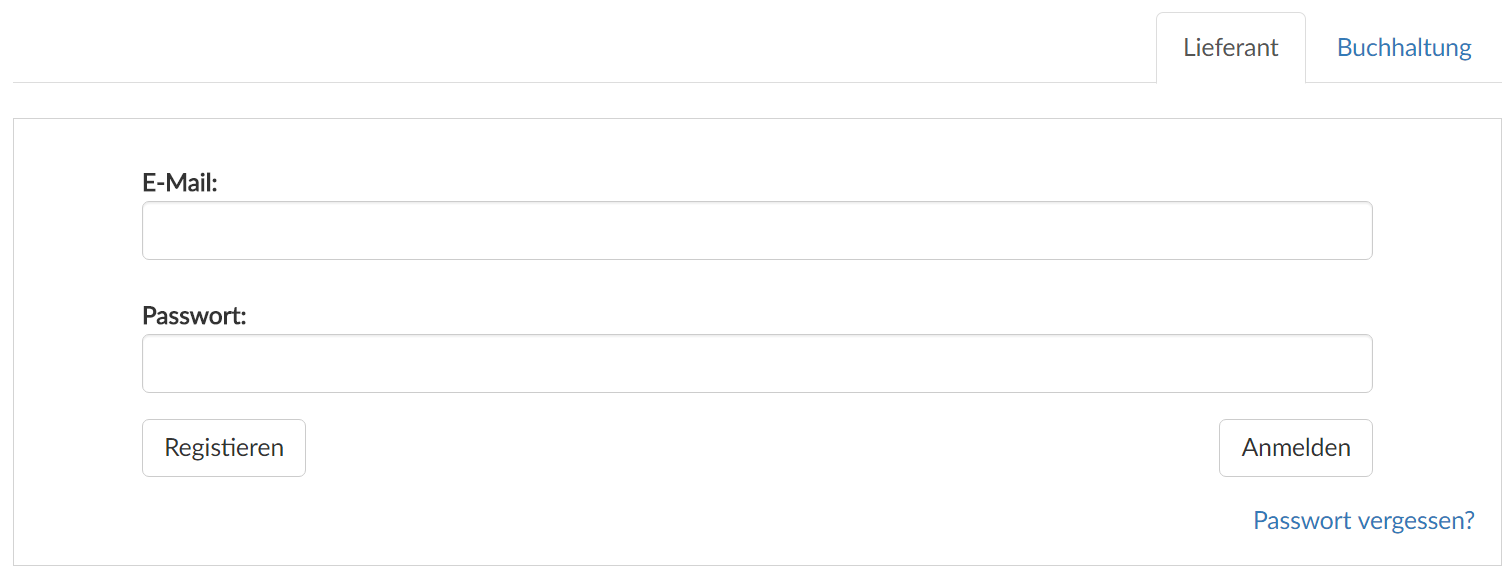
\includegraphics[width=17cm]{figures/loginmask.png}
    \label{fig:takebill}
    \caption{Login-Oberfläche Lieferant}
\end{figure}

\begin{figure}[!h]
    \centering
    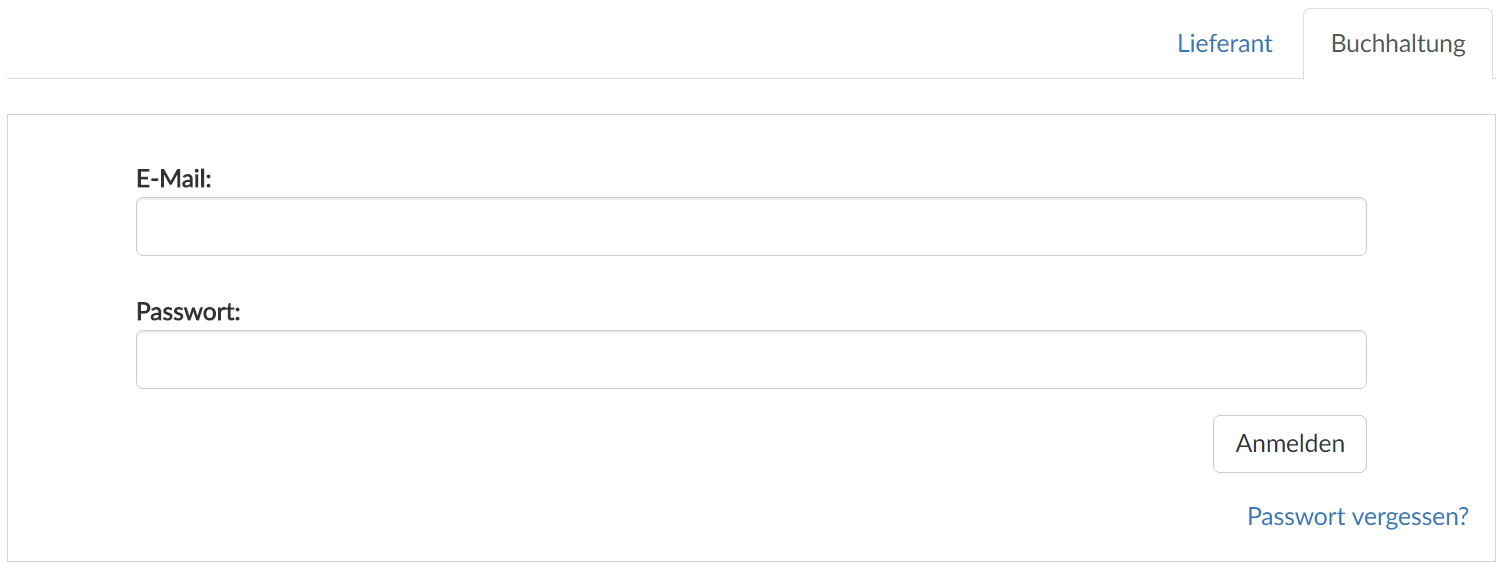
\includegraphics[width=17cm]{figures/loginbuchmock.png}
    \label{fig:takebill}
    \caption{Login-Oberfläche Buchhaltung}
\end{figure}


\newpage
In der unten stehenden Grafik ist das Ablaufdiagramm der Login-Funktion zu sehen.
\begin{figure}[!h]
    \centering
    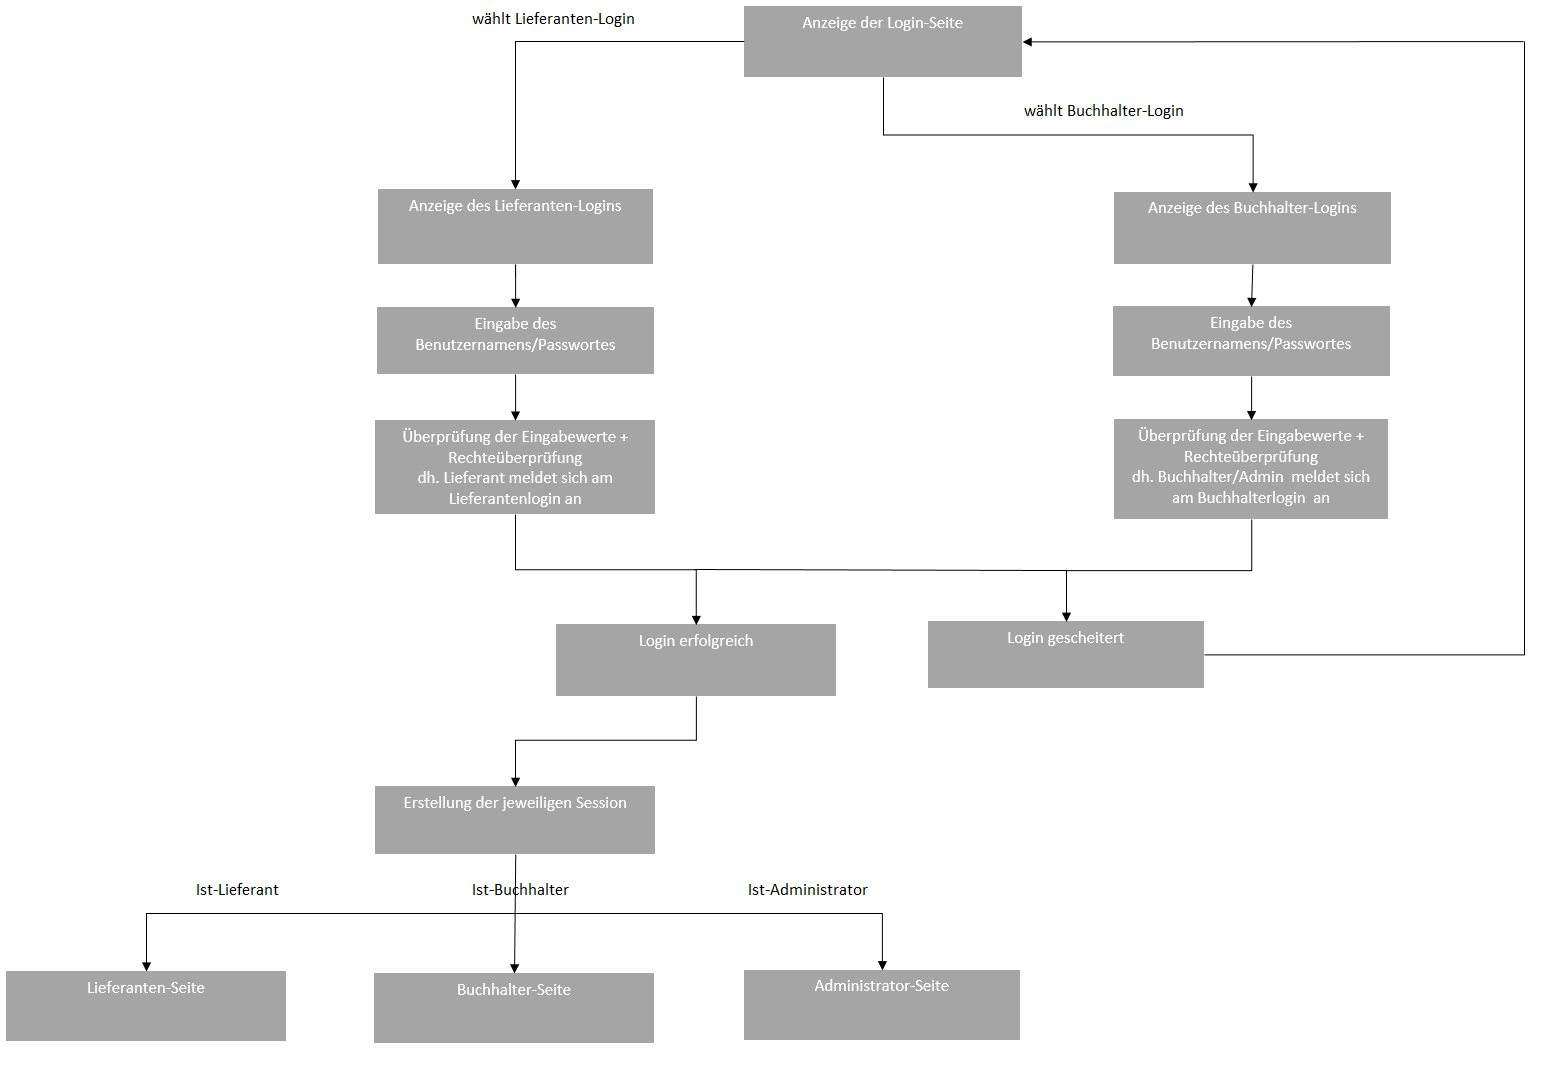
\includegraphics[width=17cm, height=15cm]{figures/login.jpg}
    \label{fig:login}
    \caption{Login-Ablaufdiagramm}
\end{figure}
\newpage

\section{Passwort vergessen}
Falls ein Benutzer (Lieferant, Buchhalter) sein Passwort vergisst, kann er dies ohne Probleme zurücksetzen. Dazu öffnet er die \glqq Passwort vergessen\grqq -Schaltfläche. Darin trägt er seine E-Mail-Adresse ein. Danach wird geprüft, ob die E-Mail-Adresse in der Datenbank existiert. Falls diese vorhanden ist, wird eine E-Mail mit einem Link zum Zurücksetzen an den jeweiligen Benutzer gesendet. Der Anwender öffnet danach seine E-Mails und gelangt auf eine Seite, auf der er sein Passwort verändern kann. Auch hier wird geprüft, ob die beiden Passwörter übereinstimmen und ob sie den Passwortkriterien der jeweiligen Benutzergruppe entsprechen. Wenn eine Überprüfung fehlschlägt, wird dem Benutzer eine entsprechende Fehlermeldung angezeigt. Falls alles erfolgreich durchgeführt wurde, wird der Anwender auf die Login-Seite weitergeleitet und er kann sich mit seinem neuen Passwort normal anmelden. 

Unten sehen Sie einen Ausschnitt aus der \glqq Passwort vergessen\grqq{} -Methode. Zuerst werden die Regeln festgelegt, denen die Eingabe entsprechen muss (Passwortkriterien, neues Passwort muss zweimal gleich eingegeben werden). Danach wird geprüft, ob die Angaben den Regeln entsprechen, wenn nicht, werden dem Benutzer die Fehler ausgegeben und falls sie stimmen wird der Benutzer zur Login-Seite weitergeleitet.

\lstset{language=PHP,caption={Passwort vergessen-Methode, für kompletten Ausschnitt siehe S. \pageref{vergessencode}},label=vergessen}
\begin{lstlisting}
$rules = array(
	'newpassword' => $criterias[0],
	'repeat_newpassword' => 'required|same:newpassword',
);

$validator = Validator::make(Input::all(), $rules, $messages);

if ($validator->fails()) {
	$messages = $validator->messages();
		return redirect()->back()->withErrors($validator);
} 
else {
	$password = $request->input('newpassword');
	User::find($id)->update(['password' => $password, 'has_changed' => 1]);
		return redirect('/');
}
\end{lstlisting}
\newpage
In den Abbildungen ist die E-Mail zu sehen, die der Benutzer erhält, wenn er sein Passwort zurücksetzen möchte, sowie die \glqq Passwort vergessen\grqq{} -Seite. 
\begin{figure}[!h]
    \centering
    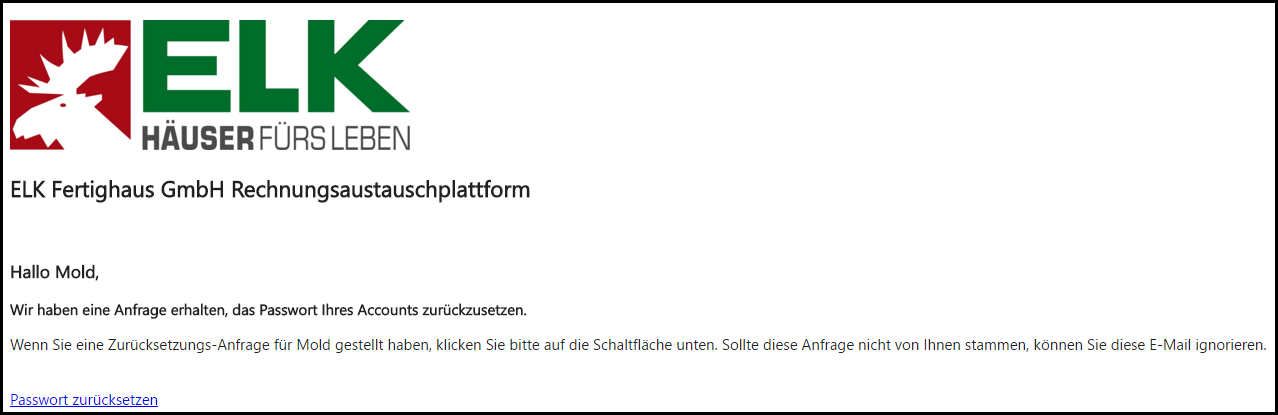
\includegraphics[width=17cm]{figures/mail.png}
    \label{fig:takebill}
    \caption{Passwort Vergessen E-Mail}
\end{figure}
\\ \\
\begin{figure}[!h]
    \centering
    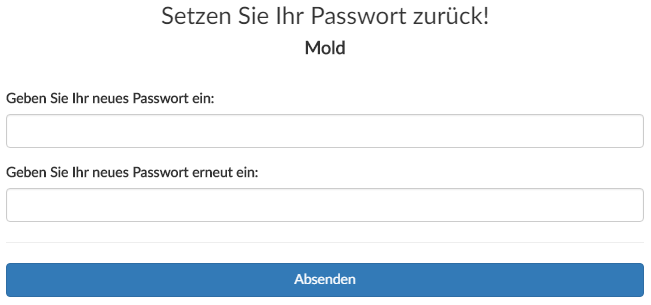
\includegraphics[width=17cm]{figures/vergessenmock.png}
    \label{fig:takebill}
    \caption{Passwort vergessen-Oberfläche}
\end{figure}

\newpage
In der unten stehenden Grafik ist das Ablaufdiagramm der \glqq Passwort vergessen\grqq{} -Funktion zu sehen.
\begin{figure}[!h]
    \centering
    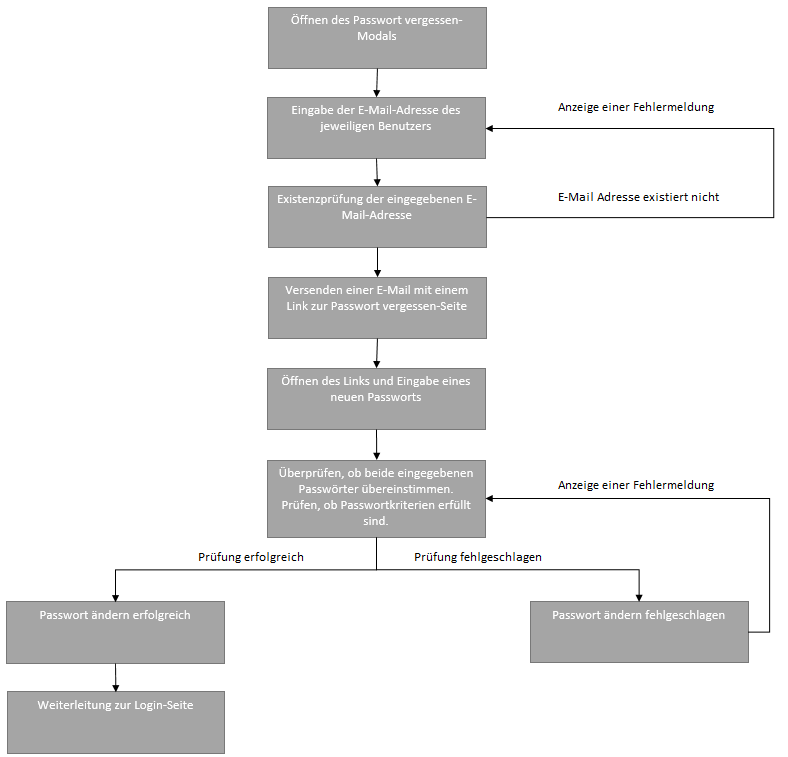
\includegraphics[width=17cm, height=15cm]{figures/vergessen.PNG}
    \label{fig:login}
    \caption{Passwort vergessen-Ablaufdiagramm}
\end{figure}
\newpage

\section{Rechnung hochladen}
Die \glqq Rechnung hochladen\grqq{}-Funktion steht nur einem Lieferanten zur Verfügung. Sie wird als zweites Tab angezeigt, neben den von ihm noch offenen Rechnungen. Zu Beginn füllt der Lieferant alle Felder des Formulars aus und wählt eine PDF, welche sich in seinem Dateiverzeichnis befinden muss, aus. Nach dem Klicken auf den Hochladen-Button werden die Größe der PDF-Datei und die eingetragenen Beträge überprüft. Erst wenn diese Felder die Kriterien erfüllen, wird die Rechnung in der Datenbank erstellt und die PDF-Datei in unserem Filesystem abgespeichert. Wenn der Vorgang erfolgreich durchgeführt wurde, wird ein weiterer Eintrag in die \glqq upload.log\grqq{} -Datei geschrieben und eine Erfolgsmeldung erscheint. Jedoch, wenn die Kriterien nicht erfüllt werden, wird eine Fehlermeldung angezeigt, die den Lieferanten bei der Fehlerausbesserung behilflich ist. \\

Ein Eintrag in der Log-Datei sieht wie folgt aus: \newline 
\textit{[2016-03-05] - [16:45:39] - [80536] - [46]}

\newpage
Hier folgt ein Code-Ausschnitt aus der \glqq Rechnung hochladen\grqq{}-Funktion. Am Beginn des Codes wird überprüft, ob alle Input-Felder ausgefüllt sind. Darauf folgt die Überprüfung, ob es sich bei der Datei um eine PDF-Datei handelt und nur dann wird der weitere Code ausgefüllt. Falls diese Kriterien erfüllt sind, wird die Rechnung in der Datenbank angelegt, die Datei hochgeladen und der PDF-Name zur Rechnung hinzugefügt. Das Loggen der Hochladen-Funktion und die Verweise auf die Seiten mit den anzuzeigenden Meldungen, die als Nächstes angezeigt werden, sind in dem Code-Fragment nicht vorhanden. Diese können im gesamten Code nachgeschlagen werden.



\lstset{language=PHP,caption={Rechnung hochladen-Funktion, für kompletten Ausschnitt siehe S. \pageref{hochladencode}},label=Rechnung-hochladen}
\begin{lstlisting}
// Die angelegten Rules nehmen und mit den Inputs prüfen
$validator = Validator::make(Input::all(), $rules, $messages);
// Wenn etwas fehlt oder fehlgeschlagen ist, dann komm ich zurück auf meine Seite mit den fehlenden Inputs
if ($validator->fails()) {
    return redirect('supplier#panel_uploadbill')->withInput()->withErrors($validator);
}

// Wenn Datei eine PDF ist
if ($pdf->getClientOriginalExtension() == 'pdf') {
    // Rechnung anlegen
    $bill = Bill::create(array(
        'amount' => $amount,
        'tax_amount' => $tax_amount,
        'document_date' => $document_date,
        'external_billnumber' => $external_billnumber,
        'billtype_id' => $billtype_id,
        'currency_id' => $currency_id,
        'company_id' => $company_id,
        'supplier_id' => $supplier_id,
        'status' => 'ready',
    ));

    // PDF-name bilden mit der ID der Rechnung
    $pdfName = $bill->id.'.'.$pdf->getClientOriginalExtension();
    // speichern der PDF
    $pdf->move('../storage/app/pdfs/', $pdfName);

    // PDF zur Rechnung hinzuspeichern
    $bill->pdf_name = $pdfName;
    $bill->save();
}
\end{lstlisting}

\newpage
In dem unten zu sehenden Formular kann ein Lieferant eine Rechnung hochladen. Dabei müssen alle Felder ausgefüllt sein.
\begin{figure}[!h]
    \centering
    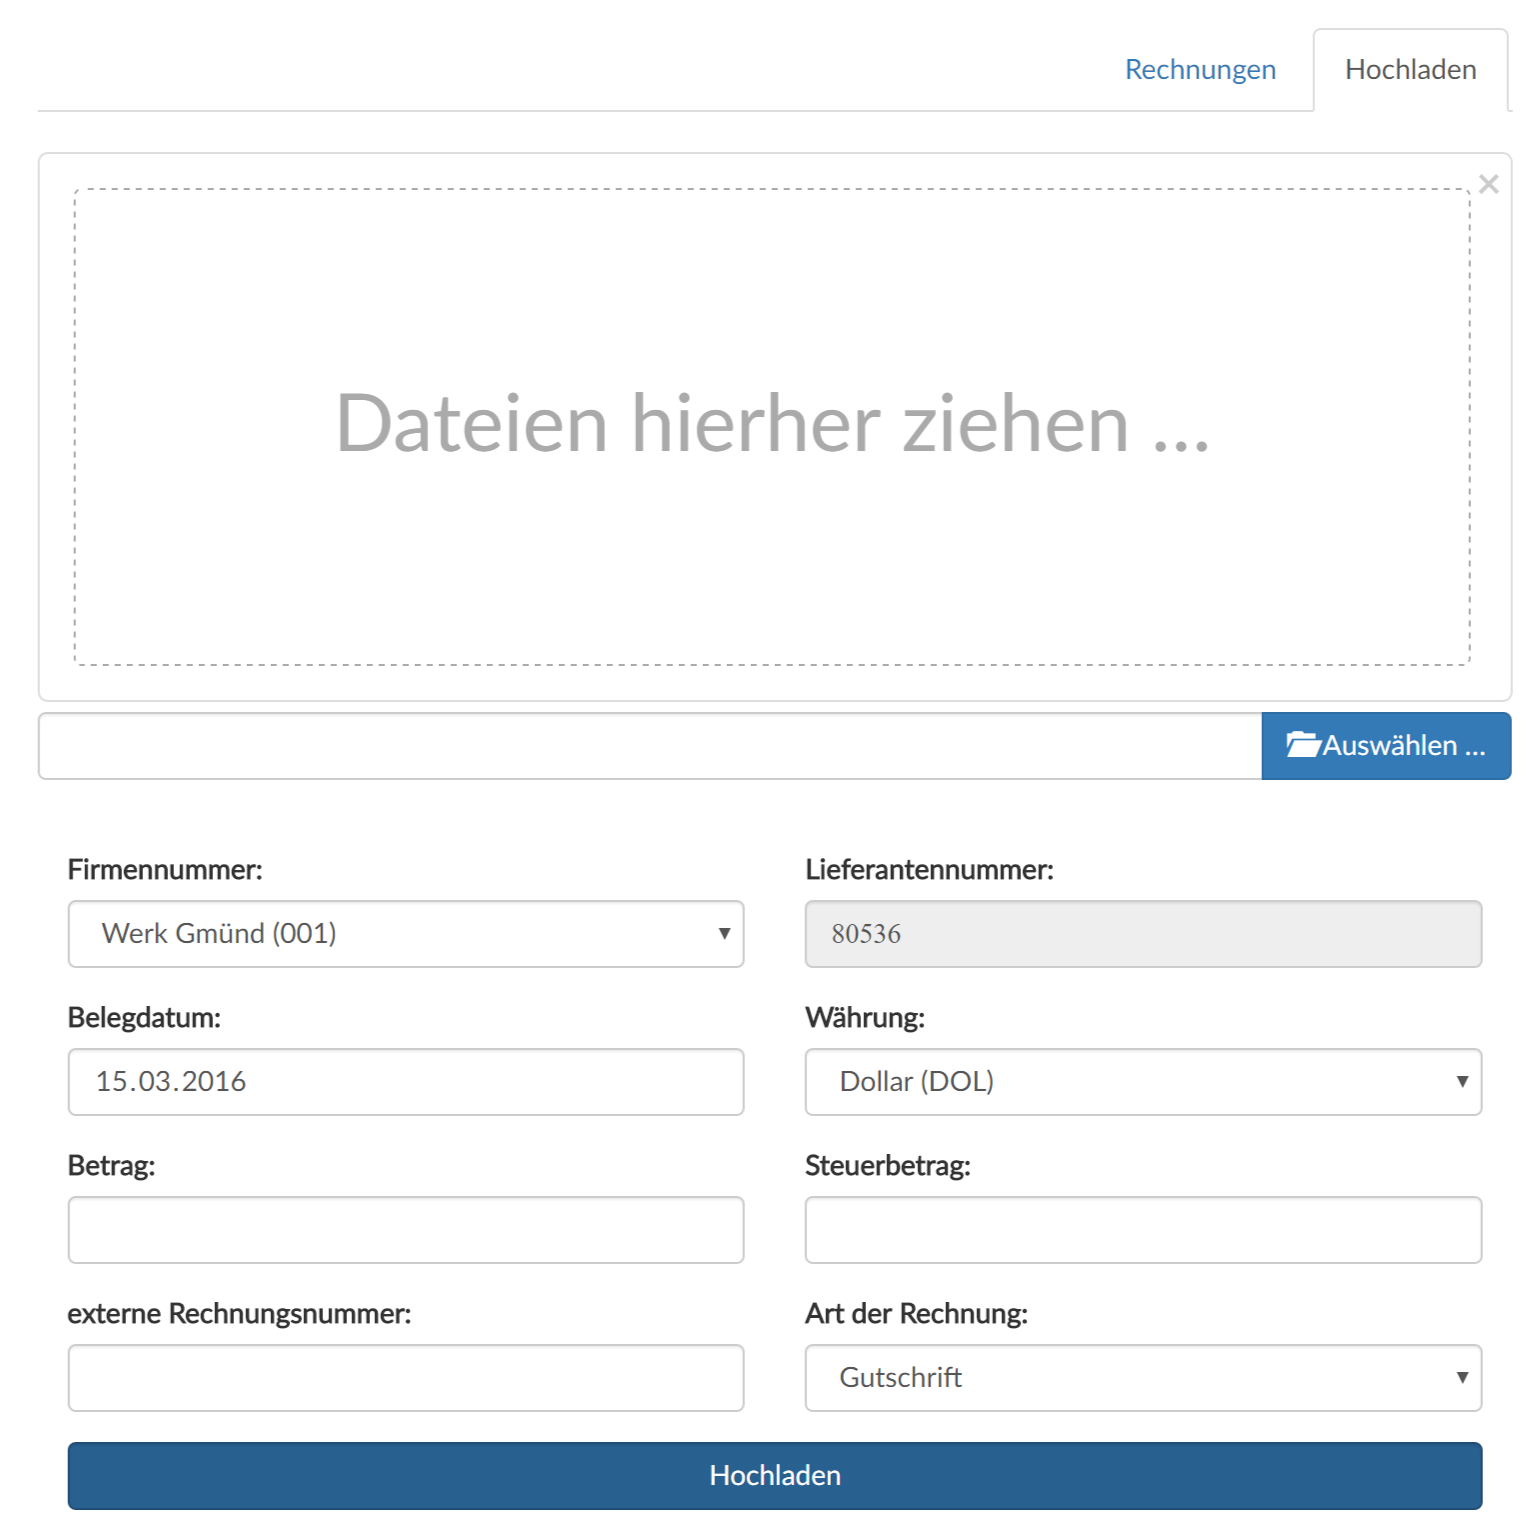
\includegraphics[width=17cm]{figures/upload.png}
    \label{fig:takebill}
    \caption{Rechnung hochladen-Oberfläche}
\end{figure}

\newpage
Das nachfolgende Bild zeigt den Ablauf der \glqq Rechnung hochladen\grqq{}-Funktion.
\begin{figure}[!h]
    \centering
    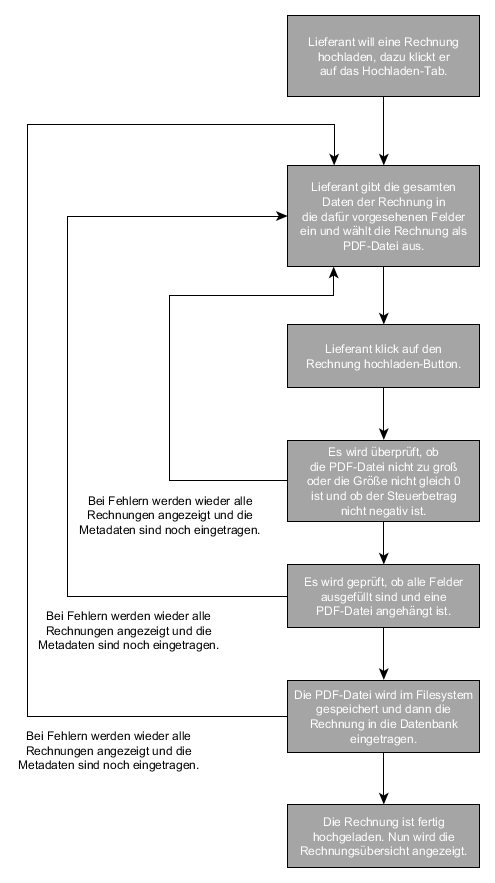
\includegraphics[width=12cm]{figures/rechnunghochladen.png}
    \label{fig:takebill}
    \caption{Rechnung hochladen-Ablaufdiagramm}
\end{figure}

\newpage

\section{Rechnung holen}
Die bereits hochgeladenen Rechnungen werden der Buchhaltung in absteigender Reihenfolge angezeigt. Wenn der Buchhalter den \glqq Rechnung holen\grqq{} -Button in der Rechnungstabelle klickt, wird zuerst eine XML-Datei aus den Metadaten der Rechnung mit den Informationen aus der Datenbank erstellt. Da die Plattform von mehreren Buchhaltern genutzt wird, wird überprüft ob die Rechnung, die geholt werden soll, bereits verarbeitet wurde. Danach wird eine E-Mail erstellt, die die XML-Datei sowie die Rechnung als PDF, die vom Lieferanten hochgeladen wurde, als Anhang besitzt. Die E-Mail wird in eine sogenannte Warteschlange geschoben und wird später versendet. Dies dient dazu, dass der aktuelle Benutzer nicht warten muss, bis die E-Mail an die rechnerunterstützte Buchhaltung versendet wurde, sondern gleich mit seiner Arbeit fortfahren kann. Alle zehn Sekunden wird eine E-Mail aus der Warteschlange entfernt und versendet. Eine Minute nachdem diejenige E-Mail mit den Anhängen versendet wurde, wird die Rechnungs PDF-Datei und die XML-Datei in ein Archiv-Verzeichnis verschoben. Außerdem wird in der Datenbank der Status \glqq geholt\grqq{} zugewiesen, daher wird diese auch nicht mehr in der Rechnungstabelle angezeigt. Des Weiteren wird ein Eintrag in der taken.log Datei erstellt. Dieser Eintrag beinhaltet das aktuelle Datum, die genaue Uhrzeit sowie die Rechnungsnummer und Lieferantennummer. Die weitere Verarbeitung der Eingangsrechnung übernimmt die computerunterstützte Buchhaltung der Firma ELK Fertighaus GmbH.
\newpage
Unten sehen Sie einen Ausschnitt aus der \glqq Rechnung holen\grqq{} -Methode. Die Methode erstellt die E-Mail und verschiebt sie in die Warteschlange. Außerdem wird der Job erstellt, der die XML-Datei und die Rechnungsdatei in ein Archiv-Verzeichnis verschiebt.

\lstset{language=PHP,caption={Rechnung holen, für kompletten Ausschnitt siehe S. \pageref{holencode}},label=holen}
\begin{lstlisting}
//Mail erstellen und Anhänge anhängen
Mail::later(10, 'mail.bill', ['billinfo' => $bill], function ($m) use ($bill, $filecontents) {
	$m->from(env('MAIL_SENDER', ''), env('MAIL_NAME', 'ELK_Rechnungsplattform'));
	$m->to($bill->email, $bill->username)->subject('Rechnungsnummer: '.$bill->id);
	$m->attach('public/pdfs/'.$bill->pdf_name);
	$m->attach('storage/app/'.$filecontents[0]);
});

//Dateien verschieben
$delete = (new SendBillEmail($bill, $filecontents))->delay(60);
$this->dispatch($delete); 
\end{lstlisting}

\vspace{1cm}
Ein Eintrag in der Log-Datei sieht wie folgt aus: \newline 
\textit{[2016-02-27] - [17:10:26] - [80536] - [5]}

\vspace{1cm}
In der Abbildung unten ist die Oberfläche zu sehen, wo der Buchhalter die Rechnung holen kann.
\begin{figure}[!h]
    \centering
    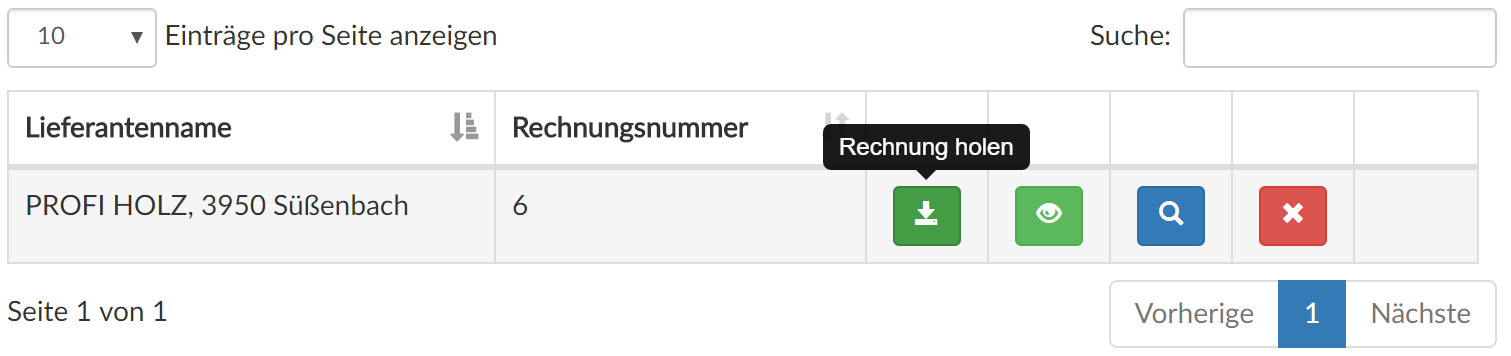
\includegraphics[width=15cm]{figures/holencode.png}
    \label{fig:takebill}
    \caption{Rechnung holen-Oberfläche}
\end{figure}

\newpage
Der folgende Ausschnitt zeigt und beschreibt den Aufbau der XML-Datei, die der Buchhaltung zugesendet wird. Weiters ist eine Beschreibung der einzelnen Elemente gegeben.
\lstset{
  language=XML,
  morekeywords={encoding,
    INVOIC02, IDOC, E1EDKA1, E1EDK03, E1EDK01, E1EDS01},
    caption={Generierte XML-Datei},label=billxml
}
\begin{lstlisting}
<?xml version="1.0" encoding="UTF-8" standalone="no"?>
<INVOIC02>
  <IDOC BEGIN="1">
    <E1EDKA1 SEGMENT="1">
      	<PARVW>RE</PARVW>	-> Rechnungsempfänger
      	<LIFNR>001</LIFNR> 	-> Standort (001 = ELK Österreich)
    </E1EDKA1>
    <E1EDKA1 SEGMENT="1">
      	<PARVW>BK</PARVW>	-> Rechnungssteller
      	<LIFNR>80536</LIFNR>	-> ELK Lieferantennummer
    </E1EDKA1>
    <E1EDK03 SEGMENT="1">
      	<IDDAT>012</IDDAT>	-> Datumsformat
      	<DATUM>20160305</DATUM>	-> Datum der Rechnung
    </E1EDK03>
    <E1EDK01 SEGMENT="1">
      	<CURCY>EUR</CURCY>	-> Währung
      	<BELNR>888</BELNR>	-> Belegnummer
      	<BSART>G</BSART>	-> Art der Rechnung z.B.: Gutschrift
    </E1EDK01>
    <E1EDS01 SEGMENT="1">
      	<SUMID>011</SUMID>	-> Art des Betrags z.B.: Steuerbetrag
      	<SUMME>88</SUMME>	-> Summe des Steuerbetrags
    </E1EDS01>
    <E1EDS01 SEGMENT="1">
      	<SUMID>005</SUMID>	-> Art des Betrags z.B.: Rechnungsbetrag
      	<SUMME>88</SUMME>	-> Summe des Rechnungsbetrags
    </E1EDS01>
  </IDOC>
</INVOIC02>
\end{lstlisting}
\newpage
In der unten stehenden Grafik ist das Ablaufdiagramm der \glqq Rechnung holen\grqq{} -Funktion zu sehen.
\begin{figure}[!h]
    \centering
    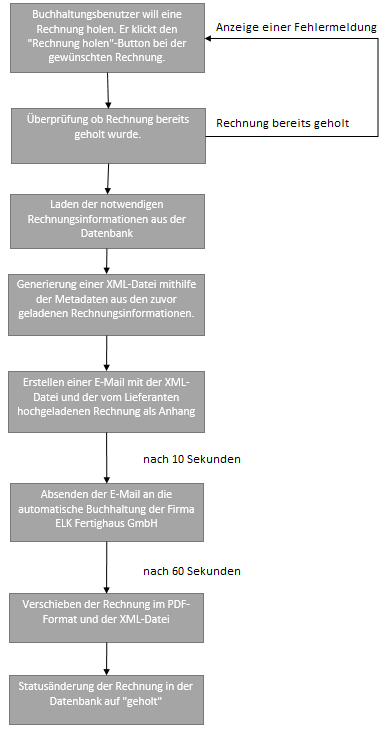
\includegraphics[width=10cm]{figures/billtaken.png}
    \label{fig:takebill}
    \caption{Rechnung holen-Ablaufdiagramm}
\end{figure}
\newpage

\section{Datenbank-Synchronisation}
Die Datenbank-Synchronisation wird automatisch durch einen Cronjob aufgerufen.

Den Cronjob selbst führt das System jede Minute aus, doch die Datenbank synchronisiert sich nur um Mitternacht. Laravel stellt ein Feature zur Verfügung, das durch einen Cronjob aufgerufen wird. In diesem Feature gibt man an, zu welcher Uhrzeit eine ausprogrammierte Funktion (z.B.: Datenbank-Synchronisation) aufgerufen werden soll.

Durch die Datenbank-Synchronisation werden die Lieferanten-Daten der Rechnungsplattform-Datenbank mit er Datenbank der Firma ELK abgeglichen und gleichgestellt. Die Excel-Datei, in der die Lieferanten-Daten der Firma ELK gespeichert sind, muss von den Datenbankexperten des Unternehmens jeden Tag erneuert werden, um eine Gleichheit der Datenbanken zu gewährleisten. Falls während der Synchronisation ein Fehler auftritt, wird der Vorgang abgebrochen und die Datenbank auf den zuvor herrschenden Stand zurückgesetzt.

Zu Beginn der Durchführung werden alle Lieferanten-Daten der Datenbank in eine Variable gespeichert und danach gelöscht. Die Benutzer, welche über Lieferanten-Rechte verfügen, werden von der Plattform gesperrt und die Excel-Datei wird eingelesen. Danach durchläuft die Funktion jeden einzelnen Eintrag der Excel-Datei und fügt diesen in die Datenbank ein. Falls einer der Lieferanten bereits einen Benutzer zugewiesen hat, wird dieser ebenfalls eingetragen und der Gesperrt-Status auf den, der vorher eingetragen war, geändert.

\newpage
Hier folgt ein Ausschnitt aus dem Code. Vor diesem Teil werden alle Lieferanten in eine Variable gespeichert und gelöscht. Außerdem speichert man die Benutzer ebenfalls ab und sperrt diese. Im Codestück wird die Excel-Datei mit den Lieferanten-Daten ausgelesen und verarbeitet. Danach legt die Funktion die einzelnen Lieferanten an und weist einen Benutzer zu, falls einer für diesen Lieferanten vorhanden ist. Nach dem Ausschnitt werden noch alle nicht gebrauchten Lieferanten-Benutzer aus der Datenbank gelöscht.
\lstset{language=PHP,caption={Datenbank-Synchronisation, für kompletten Ausschnitt siehe S. \pageref{datenbanksynchronisationcode}},label=Datenbank-Synchronisation}
\begin{lstlisting}
$file = storage_path('app').'\xlsxs\lieferanten.xlsx'; //Dateiname angeben
// Excel-Datei mithilfe des Plugins "Excel-Laravel" auslesen
$results = Excel::selectSheetsByIndex(0)->load($file, 'UTF-8')->get(array('adr_nr', 'adr_name', 'adr_uid'));
// Alle Einträge der Datei durchlaufen
foreach ($results as $row) {
    $supplier = new Supplier();
    $supplier->id = $row->adr_nr;
    $supplier->adr_name = $row->adr_name;
    $supplier->adr_uid = $row->adr_uid;

    if ($oldSup->contains('id', $row->adr_nr) == true) {
        // die alten Lieferanten durchgehen
        foreach ($oldSup as $item) {
            // schauen, wo die ADR_NR der alten Lieferanten gleich dem neuen ADR_NR ist
            if ($item->id == $row->adr_nr) {
                $supplier->user_id = $item->user_id;
                $supplier->newRegistered = $item->newregistered;

                // alle LieferantenUser durchgehen
                foreach($oldUser as $item2){
                    // Wenn die ID vom Benutzer gleich der ist, zu welchen er gehört
                    if($item2->id == $item->user_id){
                        // Benutzer sperren oder freischalten
                        User::where('id', $item->user_id)->update(['locked' => $item2->locked]);
                    }
                }
            }
        }
    }
    $supplier->save();
}
\end{lstlisting}
\newpage
Unten ist noch die Fehlerbehandlung ersichtlich. Diese wird ausgeführt, falls ein Fehler während des Auslesevorgangs, der Erstellung der Lieferanten oder der Bearbeitung der Benutzer auftritt. Im Allgemeinen dient dieser Code dazu, dass die Datenbank wieder den vorher herrschenden Stand zurückerlangt.
\lstset{language=PHP,caption={Datenbank-Synchronisation Fehlerbehandlung, für kompletten Ausschnitt siehe S. \pageref{datenbanksynchronisationfehlerbehandlungcode}},label=Datenbank-Synchronisation Fehlerbehandlung}
\begin{lstlisting}
// Falls etwas fehlschlägt
User::where('rights', 'supplier')->delete();
foreach($oldUser as $item){
    User::where('id', $item->id)->update(['locked' => $item->locked]);
}
Supplier::whereNotNull('id')->delete();
foreach($oldSup as $item){
    $item->save();
}
$this->error('Die Datenbank wurde nicht synchronisiert, da ein Fehler aufgetreten ist.');
\end{lstlisting}

\newpage
Hier ist das Ablaufdiagramm der oben beschriebenen Datenbanksynchronisation angeführt.
\begin{figure}[!h]
    \centering
    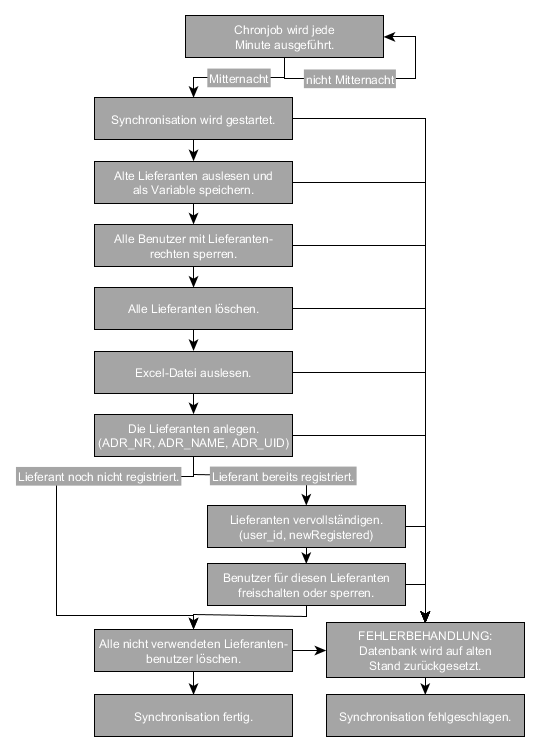
\includegraphics[width=15cm]{figures/DatenbankSynchronisieren.png}
    \label{fig:datenbanksynchronisation}
    \caption{Datenbanksynchronisation-Ablaufdiagramm}
\end{figure}
\newpage

\section{Backend-Administratoransicht}
Das Backend dient dazu, die gesamte Plattform zu verwalten. Man kann es auch als Administrator-Bereich ansehen, da das Backend nur für eine Person bestimmt ist. Der Benutzer, welcher in diesen Bereich gelangt, ist in der Datenbank bereits vorhanden und wird so mit ausgeliefert. Diese Ansicht kann erreicht werden, indem sich der Mitarbeiter mit den Anmeldedaten des Administrators am Buchhalter-Login anmeldet. Durch diese Anmeldung wird er sofort zur Administration umgeleitet.

Der Bereich beinhaltet folgende Komponenten:
\subsection{Startseite}
Wenn der Benutzer in den Administrator-Bereich gelangt, wird eine Startseite angezeigt. Auf dieser Seite werden die vier wichtigsten Daten der Plattform angezeigt. Bei den wichtigsten Daten handelt es sich um die Anzahl der registrierten Lieferanten, die Anzahl der freigeschalteten Lieferanten, die Anzahl der neuen Lieferanten und die Anzahl der offenen Rechnungen.
\begin{figure}[!h]
    \centering
    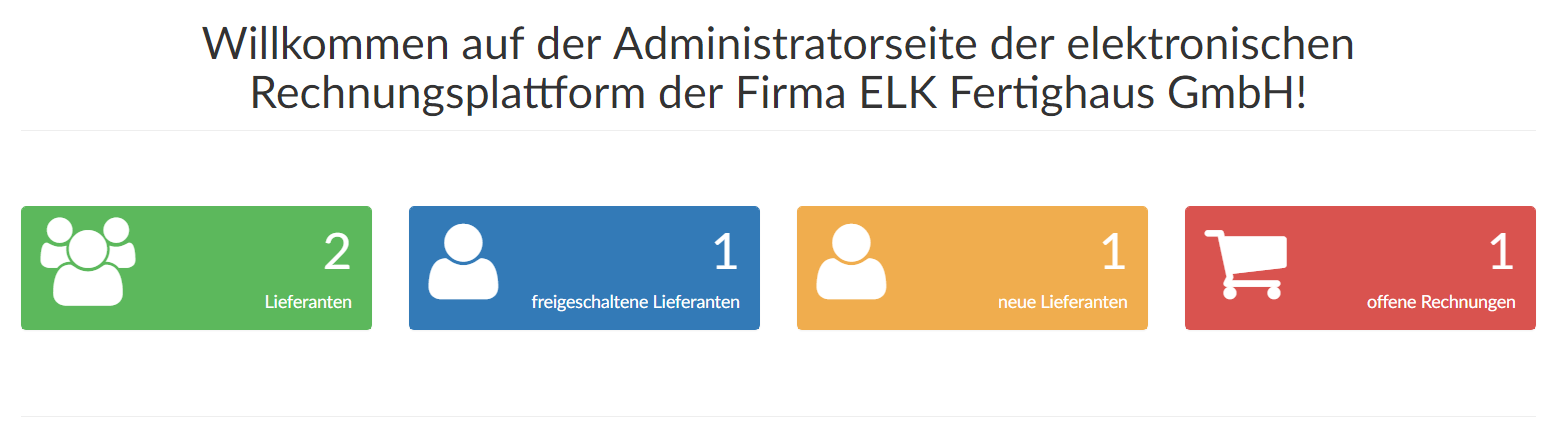
\includegraphics[width=15cm]{figures/backend.png}
    \label{fig:backendstartseite}
    \caption{Backend-Startseite}
\end{figure}
\newpage
\subsection{Lieferanten-Verwaltung}
In der Lieferanten-Verwaltung werden alle neu registrierten, registrierten und freigeschalteten Lieferanten angezeigt. Der Administrator besitzt die Rechte, dass er Lieferanten freischaltet, sperrt oder ganz löscht. Wenn der Administrations-Benutzer eine der Funktionen ausführt, wird der dazugehörige Lieferant über diese Durchführung informiert. Die Information erfolgt über eine E-Mail.
\begin{figure}[!h]
    \centering
    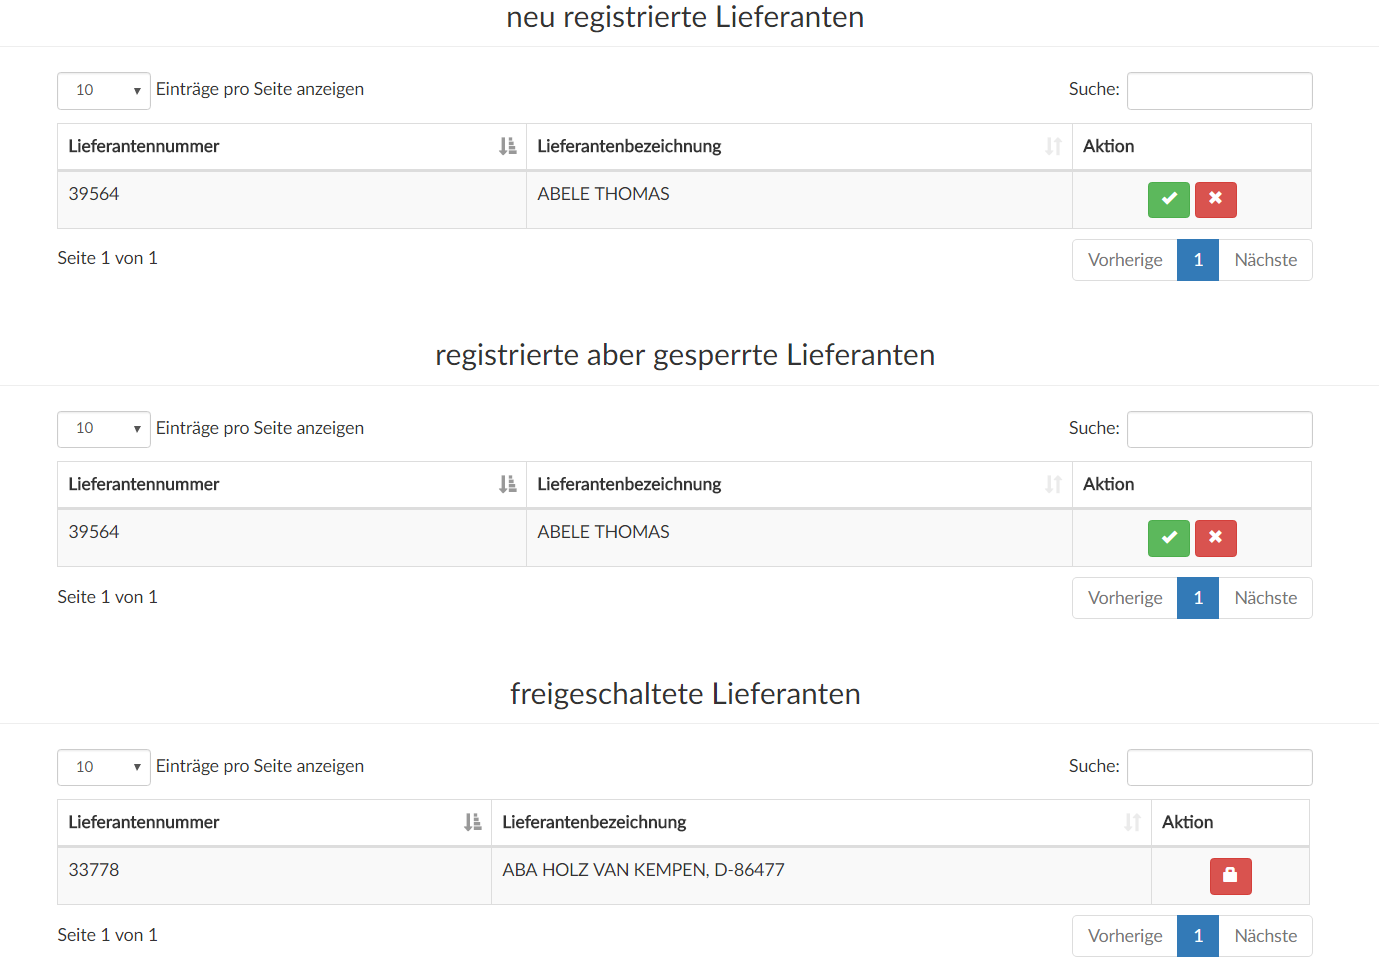
\includegraphics[width=17cm]{figures/lieferant.png}
    \label{fig:lieferantenverwaltung}
    \caption{Lieferanten-Verwaltung}
\end{figure}
\newpage
\subsection{Buchhaltungs-Verwaltung}
Die Buchhaltungs-Verwaltung dient dazu, mehrere Buchhalter für die Rechnungsplattform zu erstellen. (Im Gegensatz zur ursprünglichen Zielsetzung eines gemeinsamen Buchhalter-Nutzers.) Die einzelnen Buchhalter benötigen einen Benutzernamen und eine E-Mail. Über die angegebene E-Mail werden sie über das Erstellen benachrichtigt. Ebenfalls ist es dem Administrator möglich, die Buchhalter zu verwalten, das bedeutet, dass er die erstellten Benutzer freischalten, sperren und auch wieder löschen kann. Bei einem solchen Ereignis wird wieder eine Benachrichtigungs-E-Mail versendet.
\begin{figure}[!h]
    \centering
    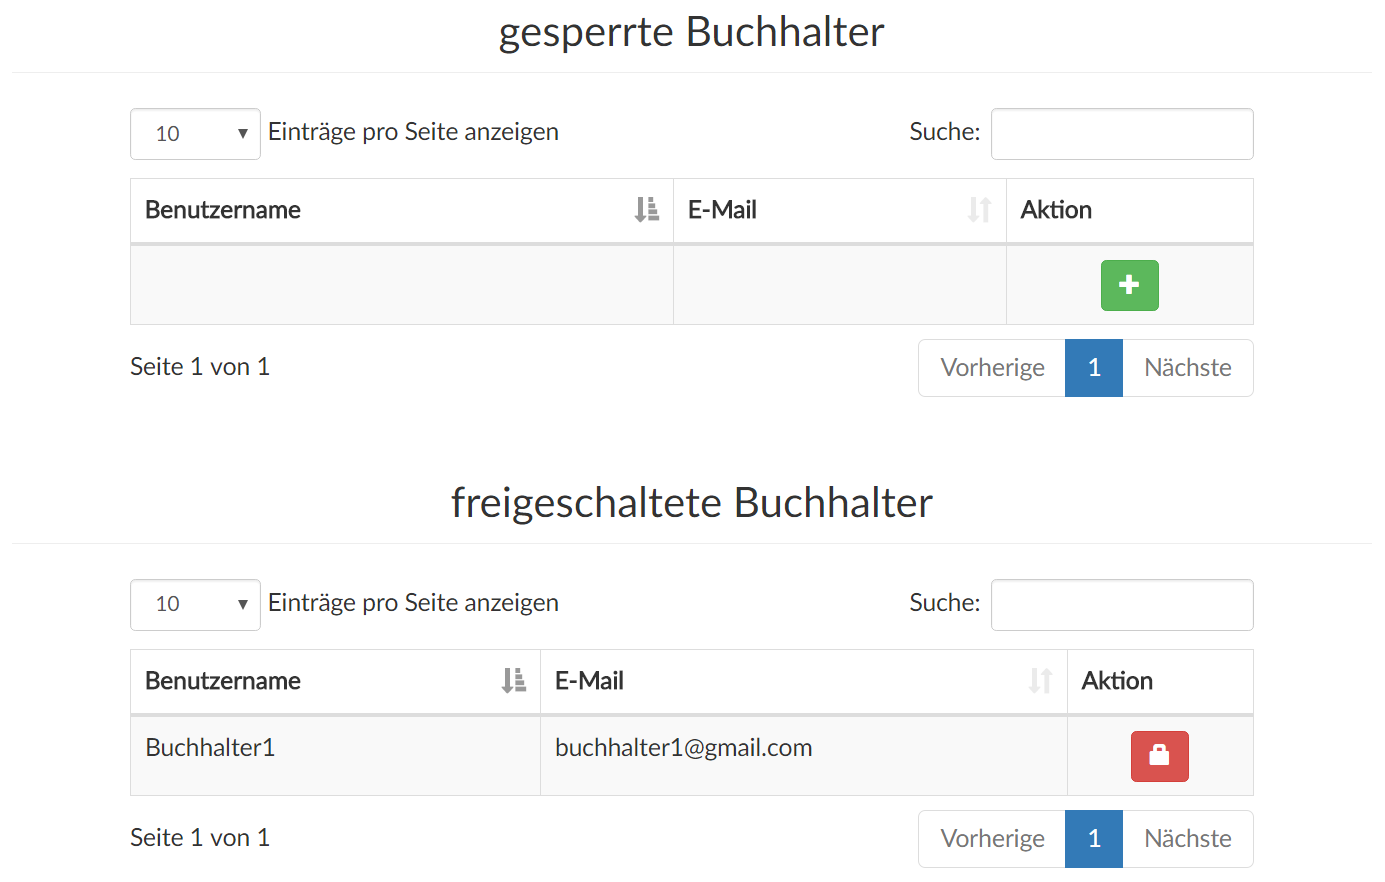
\includegraphics[width=17cm]{figures/buchhalter.png}
    \label{fig:buchhaltungsverwaltung}
    \caption{Buchhaltungs-Verwaltung}
\end{figure}
\newpage
\subsection{Passwort-Verwaltung}
Bei der Passwort-Verwaltung ist dem Administrator freigestellt, welche der vordefinierten Kriterien die Passwörter erfüllen müssen. Es ist auch möglich, die Vorgaben für die Buchhaltung, die Lieferanten und den Administrator getrennt zu definieren, wodurch eine unterschiedliche Sicherheitsstufe der Passwörter erreicht werden kann. Außerdem kann das Intervall, in welchem die Passwörter geändert werden müssen, festgelegt werden. Der Wert für die regelmäßige Änderung erstreckt sich von einer Woche bis zu höchstens fünf Wochen.
\begin{figure}[!h]
    \centering
    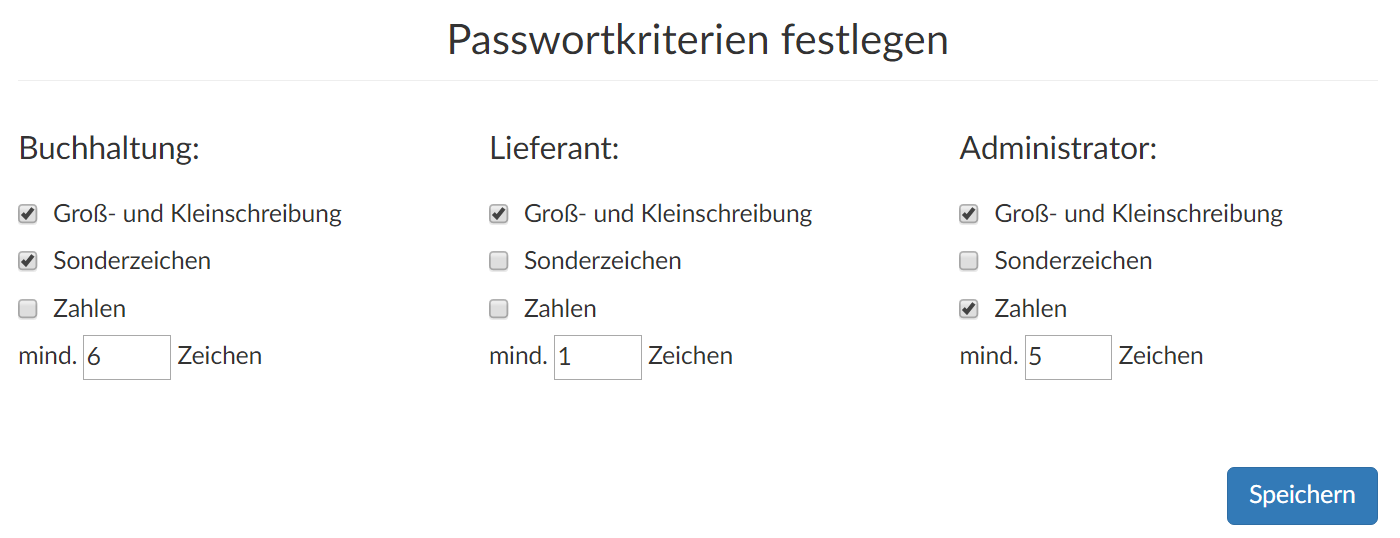
\includegraphics[width=15cm]{figures/kriterien.png}
    \label{fig:passwortkriterien}
    \caption{Passwortkriterien}
\end{figure}
\begin{figure}[!h]
    \centering
    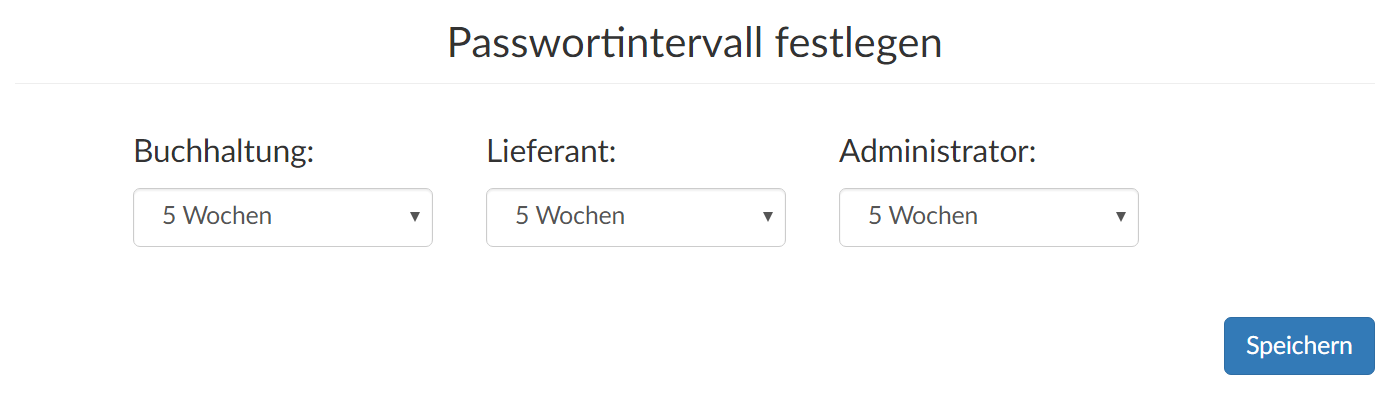
\includegraphics[width=15cm]{figures/intervall.png}
    \label{fig:passwortintervall}
    \caption{Passwort-Änderungsintervall}
\end{figure}
\newpage
\subsection{Standorte-Verwaltung}
Mit der Standorte-Verwaltung können neue Standorte der Firma hinzugefügt oder die bestehenden bearbeitet werden. Nach dem Erstellen eines Standortes ist es nicht möglich die Standort-Nummer zu verändern, sondern nur die Firmenbezeichnung. Löschen kann man keine Firma, denn sonst würden vielleicht Rechnungsdaten fehlen.
\begin{figure}[!h]
    \centering
    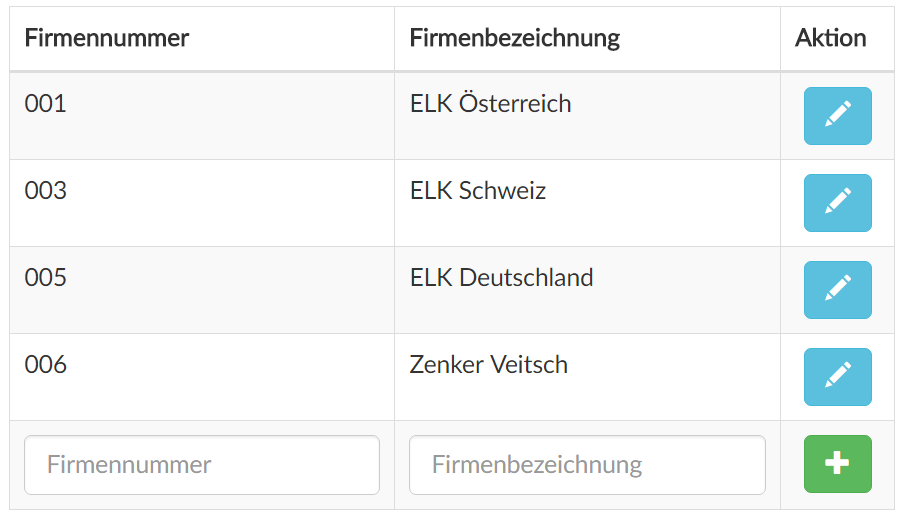
\includegraphics[width=15cm]{figures/standorte.png}
    \label{fig:standorteverwaltung}
    \caption{Standorte-Verwaltung}
\end{figure}
\newpage
\subsection{Währungs-Verwaltung}
Hier verwaltet der Administrator die Währungen, die eine Rechnung, Gutschrift und so weiter, aufweisen darf. Die verschiedenen Währungen können nur erstellt und bearbeitet werden.
\begin{figure}[!h]
    \centering
    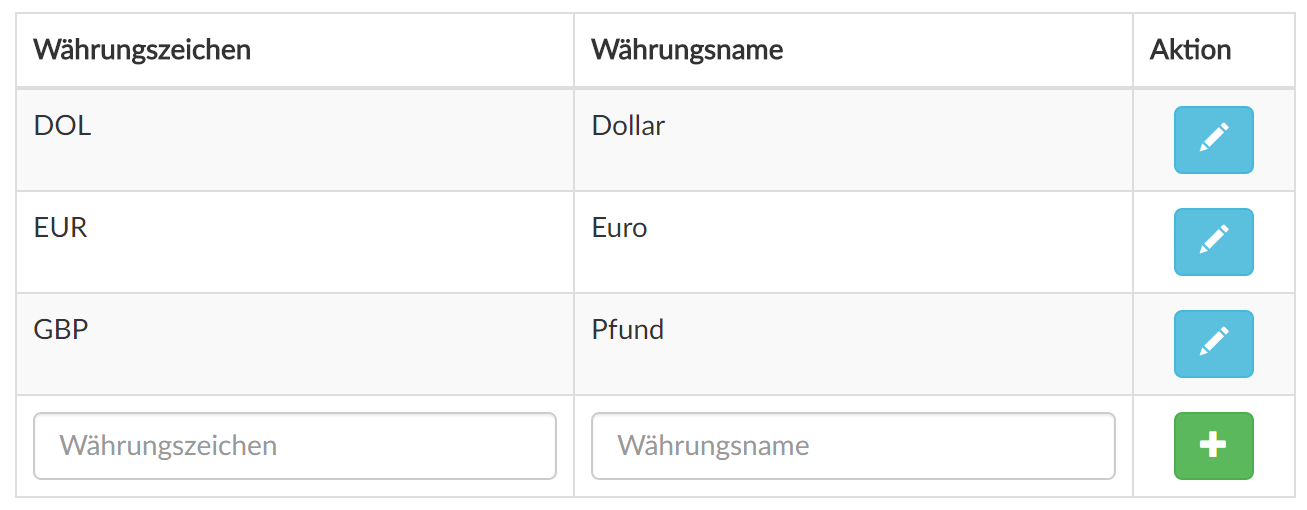
\includegraphics[width=15cm]{figures/waehrungen.png}
    \label{fig:waehrungsverwaltung}
    \caption{Währungs-Verwaltung}
\end{figure}

\subsection{Rechnungsarten-Verwaltung}
Auf dieser Ansicht können die Rechnungsarten erstellt und bearbeitet werden. Jede Art, die in dieser Übersicht angezeigt wird, kann beim Erstellen einer Rechnung vom Lieferanten ausgewählt werden. Die Löschen-Funktion ist nicht vorhanden, da beim Löschen Daten bei den bereits hochgeladenen Rechnungen fehlen könnten.
\begin{figure}[!h]
    \centering
    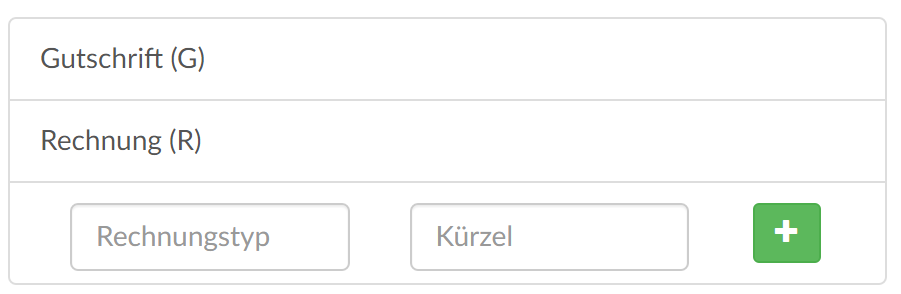
\includegraphics[width=15cm]{figures/rechnungsarten.png}
    \label{fig:rechnungsartenverwaltung}
    \caption{Rechnungsarten-Verwaltung}
\end{figure}
\newpage
\subsection{E-Mail-Verwaltung}
Mit der E-Mail-Verwaltung ist es dem Administrator möglich, die Benachrichtigungs-E-Mails zu verändern. An dieser Oberfläche gibt es drei Adressen zu verwalten. Die erste ist die wichtigste der gesamten Plattform, nämlich die des automatisierten Rechnungssystems. Auf diese E-Mail werden alle geholten Rechnungen gesendet. Die zweite wird benötigt, um die Buchhaltung über fehlerhafte Rechnungen zu informieren. Jedoch ist die Benachrichtigung auch in der Buchhalter-Oberfläche bei der Rechnungsübersicht erkennbar. Bei der dritten E-Mail handelt es sich um die, auf welche der Administrator zugreift. Auf diese E-Mail wird eine Benachrichtigung gesendet, wenn sich ein neuer Lieferant registriert.
\begin{figure}[!h]
    \centering
    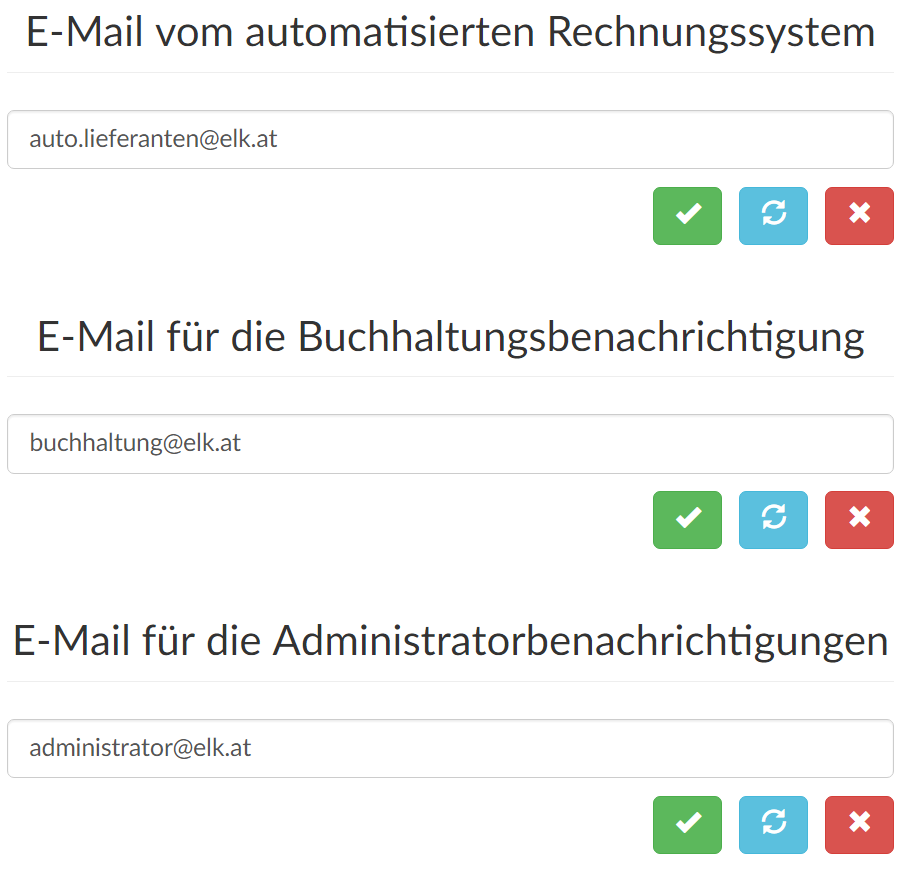
\includegraphics[width=15cm]{figures/emails.png}
    \label{fig:emailsverwaltung}
    \caption{E-Mail-Verwaltung}
\end{figure}ft. Auf diese E-Mail wird eine Benachrichtigung gesendet, wenn sich ein neuer Lieferant anmeldet.
\begin{figure}[!h]
    \centering
    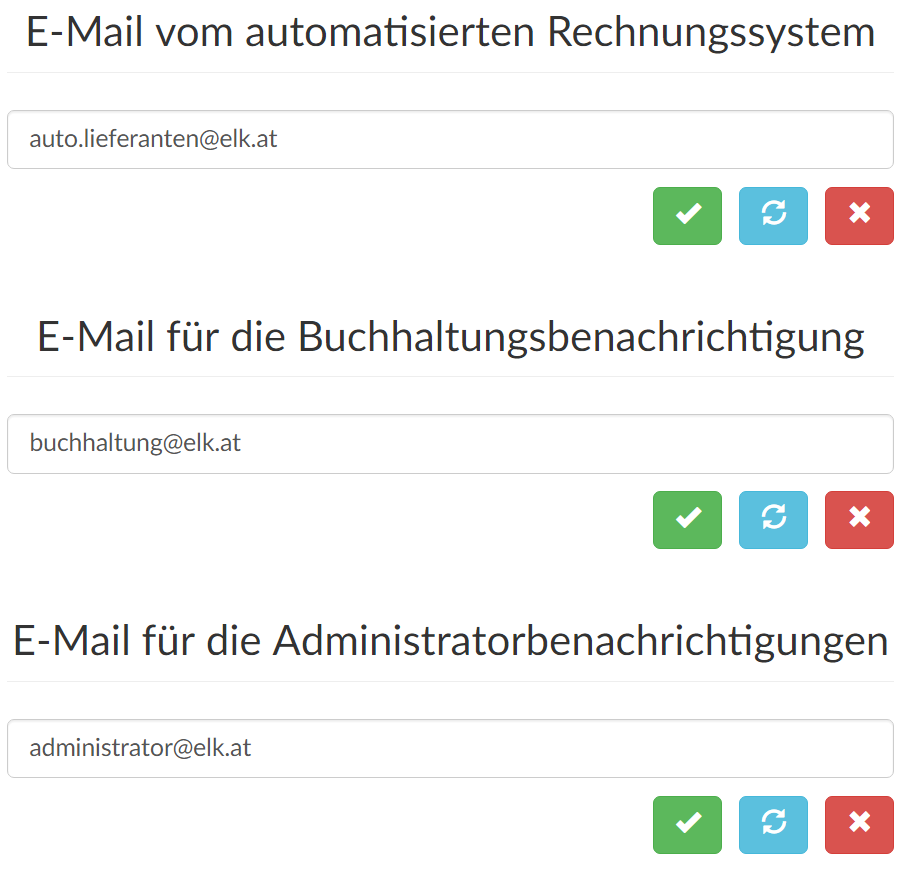
\includegraphics[width=15cm]{figures/emails.png}
    \label{fig:emailsverwaltung}
    \caption{E-Mails-Verwaltung}
\end{figure}